\chapter{Arrays of Arrays}

The last two chapters of this book use 2D graphics to illustrate advanced object-oriented concepts.
If you haven't yet read Appendix~\ref{graphics}, you might want to read it now and get familiar with the \java{Canvas}, \java{Color}, and \java{Graphics} classes from the \java{java.awt} package.

In this chapter we use these classes to draw images and animations, and to run graphical simulations.


\section{Conway's Game of Life}

``The Game of Life'', or GoL for short, was developed John H. Conway and popularized in 1970 in Martin Gardner’s column in Scientific American.
Conway calls it a ``zero-player game'' because no players are needed to choose strategies or make decisions.
After you set up the initial conditions, you watch the game play itself.
That turns out to be more interesting than it sounds; you can read about it at \url{http://en.wikipedia.org/wiki/Conway's_Game_of_Life}.

\begin{figure}[!ht]
\begin{center}
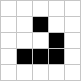
\includegraphics{figs/glider.png}
\caption{A ``Glider'' in the Game of Life.}
\label{fig:glider}
\end{center}
\end{figure}

The game board is a two-dimensional grid of square cells.
Each cell is either ``alive'' or ``dead''; the color of the cell indicates its status.
Figure~\ref{fig:glider} shows an example grid configuration.

\index{neighbor}

The game proceeds in time steps, during which every cell interacts with the neighbors in the eight adjacent cells.
At each step, the following rules are applied:

\begin{enumerate}
\item A live cell with fewer than two live neighbors dies, as if by underpopulation.
\item A live cell with more than three live neighbors dies, as if by overpopulation.
\item A dead cell with exactly three live neighbors becomes a live cell, as if by reproduction.
\end{enumerate}

\index{stable configuration}

Notice some consequences of these rules.
If you start with a single live cell, it dies.
If all cells are dead, no cells come to life.
But if you have four cells in a square, they keep each other alive, so that's a stable configuration.

Another initial configuration is shown in Figure~\ref{fig:blinker}.
If you start with three horizontal cells, the center cell lives, the left and right cells die, and the top and bottom cells come to life.
The result is three vertical cells.

During the next time step, the center cell lives, the top and bottom cells die, and the left and right cells come to life.
The result is three horizontal cells, so we're back where we started, and the pattern repeats forever.

\begin{figure}[!ht]
\begin{center}
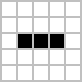
\includegraphics{figs/blinker-0.png}
\raisebox{38pt}{~$\longrightarrow$~}
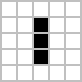
\includegraphics{figs/blinker-1.png}
\raisebox{38pt}{~$\longrightarrow$~}
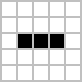
\includegraphics{figs/blinker-0.png}
\raisebox{38pt}{~$\longrightarrow$~ \ldots}
\caption{A ``Blinker'' in the Game of Life.}
\label{fig:blinker}
\end{center}
\end{figure}

Patterns like this are called ``periodic'', because they repeat after a period of 2 or more time steps.
But they are also considered stable, because the total number of live cells doesn't grow over time.

Most simple starting configurations either die out quickly or reach a stable configuration.
But there are a few starting conditions that display remarkable complexity.
One of those is the R-pentomino: it starts with only five cells, runs for 1103 time steps, and ends in a stable configuration with 116 live cells (see \url{http://www.conwaylife.com/wiki/R-pentomino}).

In the following sections, we implement the Game of Life in Java.


\section{The Cell Class}

% I don't think we can really say we need three classes; it's just a design choice we made.

We'll organize the code in three classes: one for cells, one for the grid, and one for the game itself.
We'll start with the cells.

To draw a cell, we need to know its coordinates on the screen.
We could use a \java{Rectangle} object (see Section~\ref{sec:Rectangle}) to store the cell's coordinates.
However, since the cells are square (not rectangular), we can represent their locations with three integers: the \java{x} and \java{y} coordinates of the upper-left corner, and the \java{size} of the square (length of each side).
Each cell also needs a \java{Color} to represent its state: alive or dead.

Here is the beginning of the \java{Cell} class:

\begin{code}
public class Cell {
    private final int x;
    private final int y;
    private final int size;
    private Color color;
}
\end{code}

Notice that \java{x}, \java{y}, and \java{size} are constants.
Once the cell is created, we don't want it to move accidentally.
Its \java{color}, on the other hand, is not a constant and might change frequently.

% Nice!  The previous paragraph answers exactly the question I had.

The next step is to write a constructor.
Here's one that takes \java{x}, \java{y}, and \java{size} as parameters, and sets {\tt color} to a default value.

\begin{code}
public Cell(int x, int y, int size) {
    this.x = x;
    this.y = y;
    this.size = size;
    this.color = Color.WHITE;
}
\end{code}

The following line uses the constructor to create a \java{Cell}.
Its upper-left corner is at (0, 0), and the cell is 10x10 pixels.

\begin{code}
Cell cell = new Cell(0, 0, 10);
\end{code}

The following method draws a cell.
Like the \java{paint} method in Appendix~\ref{graphics},
it takes a graphics context as a parameter, which it uses to
call \java{fillRect}, which draws the center of the cell, and \java{drawRect}, which draws a gray border.

\begin{code}
public void draw(Graphics g) {
    g.setColor(this.color);
    g.fillRect(x + 1, y + 1, size - 1, size - 1);
    g.setColor(Color.LIGHT_GRAY);
    g.drawRect(x, y, size, size);
}
\end{code}

We also need methods to read and write the cell's color.
We could just provide \java{getColor} and \java{setColor},
but the code will be more readable if we provide methods more customized for the Game of Life:

\begin{code}
public static final Color OFF = Color.WHITE;
public static final Color ON = Color.BLACK;

public boolean isOn() {
    return color == ON;
}

public boolean isOff() {
    return color == OFF;
}
\end{code}

\java{isOn} and \java{isOff} check the state of the cell.

\begin{code}
public void turnOn() {
    color = ON;
}

public void turnOff() {
    color = OFF;
}
\end{code}

\java{turnOn} and \java{turnOff} modify the state of the cell.


\section{Two-Dimensional Arrays}

To represent a grid of cells, we use a 2D array.
To create a 2D array, we specify the number of rows and columns like this:

\begin{code}
int rows = 5;
int cols = 5
Cell[] array = new Cell[rows][cols];
\end{code}

The result is an array with 5 rows and 5 columns.
Initially, the elements of the array are all \java{null}.
We can fill the array with cells like this:

\begin{code}
for (int r = 0; r < rows; r++) {
    int y = r * size;
    for (int c = 0; c < cols; c++) {
        int x = c * size;
        array[r][c] = new Cell(x, y, size);
    }
}
\end{code}

The loop variables \java{r} and \java{c} are the row and column indexes of the cells.
The variables \java{x} and \java{y} are the coordinates.
For example, if \java{size} is 10 pixels, then the cell at index (1, 2) would be at coordinates (10, 20) on the screen.

In Java, a 2D array is really an array of arrays.
Or maybe it would be clearer to say it's an array of rows, and each row is an array.

%The expression \java{array[r * 5 + c]} calculates the index of the row and column in the array.
%For example, the array index of the cell at (1, 2) would be 7.
%Figure~\ref{fig:1D-array} illustrates how the rows are arranged.
%
%\begin{figure}[!ht]
%\begin{center}
%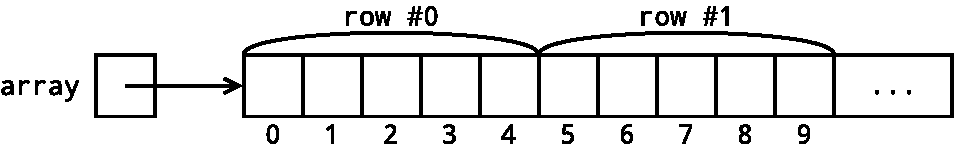
\includegraphics[width=366pt]{figs/1D-array.pdf}
%\caption{Storing rows and columns with an array.}
%\label{fig:1D-array}
%\end{center}
%\end{figure}
%
%\index{row-major order}
%\index{multidimensional array}
%
%This way of represdenting two-dimensional data is know as {\bf row-major order}, because the elements are stored row by row.
%A more natural way to represent two-dimensional data is to use {\bf multidimensional arrays}, or arrays of arrays, as shown in 

Figure~\ref{fig:2D-array} shows what it looks like.

\begin{figure}[!ht]
\begin{center}
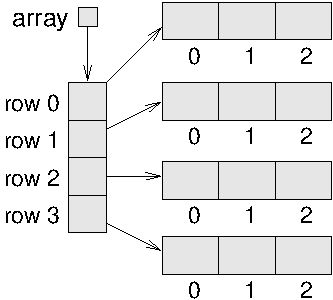
\includegraphics[width=265pt]{figs/2D-array.pdf}
\caption{Storing rows and columns with an array of arrays.}
\label{fig:2D-array}
\end{center}
\end{figure}

\java{array} is an array of references that refer to arrays of \java{Cell} objects.
When we write \java{array[r][c]}, Java uses the first index to select a row, and the second index to select an element from the row.

%
%Using arrays of arrays makes it easier to refer to individual cells by row and column indexes.
%We can rewrite the previous code by making two changes:
%
%\begin{center}
%\begin{tabular}{rl}
%Replace: & \java{Cell[] array = new Cell[25];} \\[-1ex]
%   With: & \java{Cell[][] array = new Cell[5][5];} \\[1ex]
%Replace: & \java{array[r * 5 + c] = new Cell(x, y, SIZE);} \\[-1ex]
%   With: & \java{array[r][c] = new Cell(x, y, SIZE);} \\
%\end{tabular}
%\end{center}
%
%Notice that we no longer need to calculate the index \java{r * 5 + c}.
%Instead, the expression \java{array[r]} gets the array at index \java{r}, after which \java{[c]} gets the cell at index \java{c}.


\section{The GridCanvas Class}

Now that we have a \java{Cell} class and a way of representing a two-dimensional array of cells, we can write a class to represent a grid of cells.
We encapsulate the code from the previous section and generalize it to construct a grid of any size:

\begin{code}
public class GridCanvas extends Canvas {
    private Cell[][] array;

    public GridCanvas(int rows, int cols, int size) {
        array = new Cell[rows][cols];
        for (int r = 0; r < rows; r++) {
            int y = r * size;
            for (int c = 0; c < cols; c++) {
                int x = c * size;
                array[r][c] = new Cell(x, y, size);
            }
        }

        // set the canvas size
        setSize(cols * size, rows * size);
    }
}
\end{code}

\index{IS-A}
\index{HAS-A}
\index{Graphics}

Using vocabulary from the previous chapter, \java{GridCanvas} ``is~a'' \java{Canvas} that ``has~a'' two-dimensional array of cells.
By extending the \java{Canvas} class from \java{java.awt}, we inherit methods for drawing graphics on the screen.

Now to draw the grid, we use nested loops to traverse the array:

\begin{code}
public void draw(Graphics g) {
    for (Cell[] row : array) {
        for (Cell cell : row) {
            cell.draw(g);
        }
    }
}
\end{code}

When we use a 2D array in an enhanced \java{for} loop, Java loops through the rows; each row is a 1D array.

It's helpful to read this method in English: ``For each \java{row} in the \java{array}, and for each \java{cell} in the \java{row}, draw the \java{cell} in the graphics context.''
Each cell contains its coordinates and size, so it knows how to draw itself.

Classes that extend \java{Canvas} are supposed to provide a method called \java{paint} that ``paints'' the contents of the \java{Canvas}.
It gets invoked when the \java{Canvas} is created and any time it needs to be redrawn; for example, when its window is moved or resized.

Here's the \java{paint} method for \java{GridCanvas}:

\begin{code}
public void paint(Graphics g) {
    draw(g);
}
\end{code}

When the window management system calls \java{paint}, \java{paint} calls \java{draw}, which draws the cells.

% Do we actually need update?

In additional to \java{draw} and \java{paint}, we provide methods for working with the grid itself.

\java{numRows} and \java{numCols} return the number of rows and columns.
We can get this information from the 2D array itself, using \java{length}:

\begin{code}
public int numRows() {
    return array.length;
}

public int numCols() {
    return array[0].length;
}
\end{code}

\java{numRows} returns the length of the array, which is the number of rows (remember that a 2D array is an array of rows).

\java{numCols} returns the length of the first row, which is the number of columns.

Finally, we provide methods that read and write individual cells.

\begin{code}
public Cell cellAt(int r, int c) {
    return array[r][c];
}

public void init(int r, int c) {
    array[r][c].turnOn();
}
\end{code}

\java{cellAt} looks up the \java{Cell} at row \java{r}, column \java{c}.


% TODO: Come back to this when the API is settled


\section{Starting the Game}

To encapsulate the rules of GoL, we define a third class called \java{Conway}.
The \java{Conway} class ``has~a'' \java{GridCanvas} that represents the state of the game.

The default constructor creates the \java{GridCanvas} and sets up an initial state.

\begin{code}
public class Conway {
    private GridCanvas grid;

    public Conway() {
        grid = new GridCanvas(5, 10, 20);
        grid.init(2, 1);
        grid.init(2, 2);
        grid.init(2, 3);
        grid.init(1, 7);
        grid.init(2, 7);
        grid.init(3, 7);
    }
}
\end{code}

\index{JFrame}

Before we implement the rest of the game, we'll write a \java{main} method that creates a \java{Conway} object and displays it.

We can use this method to test \java{Cell} and \java{GridCanvas}, and to develop the other methods we need.

\begin{code}
public static void main(String[] args) {
    String title = "Conway's Game of Life";
    Conway game = new Conway();
    JFrame frame = new JFrame(title);
    frame.setDefaultCloseOperation(JFrame.EXIT_ON_CLOSE);
    frame.setResizable(false);
    frame.add(game.grid);
    frame.pack();
    frame.setVisible(true);
    mainloop();
}
\end{code}

\java{main} instantiates a \java{JFrame}, which creates a window on the screen, adds the \java{GridCanvas} to the \java{Frame}, and makes it visible.
The \java{JFrame} is configured to exit the program when closed.
Resizing the window is disabled.

Figure~\ref{fig:conway} shows the result.

\begin{figure}[!ht]
\begin{center}
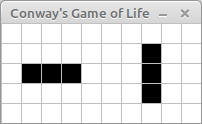
\includegraphics{figs/conway.png}
\caption{Screenshot of the initial Conway application.}
\label{fig:conway}
\end{center}
\end{figure}



\section{The mainloop}

At the end of \java{main}, we call \java{mainloop}, which uses a
\java{while} loop to simulate the time steps of the Game of Life.

\begin{code}
public static void mainloop(Conway game) {
    while (true) {
        game.update();
        game.grid.repaint();
    
        Thread.sleep(500);    // compiler error
    }
\end{code}

During each time step, we update the state of the \java{game} and repaint the \java{grid}.
(The \java{update} method will be discussed in Section~\ref{sec:update}.)

This loop will execute quickly, so we will use \java{Thread.sleep} to add a half-second delay (500 ms) after each step.

\index{Thread.sleep}
\index{sleep}

\index{InterruptedException}
\index{Exception!Interrupted}

There's just one problem: compiling this code results in the error ``unreported exception InterruptedException''.
In other words, an \java{InterruptedException} may occur while sleeping.


\section{Exception Handling}

So far the only exceptions we have seen are run-time errors like \java{ArrayIndexOutOfBoundsException} and \java{NullPointerException}.
When one of these exceptions occur, Java displays a message and ends the program.

If you don't want the program to terminate, you can ``catch'' an exception with a \java{try} statement.  Here's what it looks like:

\index{try}
\index{catch}
\index{Statement!try}
\index{Statement!catch}

\begin{code}
    try {
        Thread.sleep(500);
    } catch (InterruptedException e) {
        // do nothing
    }
\end{code}

The syntax is similar to an \java{if} statement, and the logic is, too.
First, Java runs the code in the ``try block'', which calls \java{Thread.sleep} in this example.

If an \java{InterruptedException} occurs during the try block, Java executes the ``catch block''; in this example, the catch block contains a comment, so it doesn't do anything.

If a different exception occurs during the try block, Java does whatever it would do otherwise, which is probably to display a message and end the program.

If no exceptions occur during the try block, the catch block doesn't run and the program continues.

In the example, the effect of the \java{try} statement is to ignore  \java{InterruptedException} if it occurs.

As an alternative, we could use the catch block to display a customized message, end the program, or handle the exception in whatever way is appropriate.
For example, if use input causes an exception, you could catch the exception and prompt the user to try again later.

% There's more to learn about exception handling that is beyond the scope of this book.
You can read more about exceptions in the Java tutorials at \url{https://thinkjava.org/exceptions}.


\section{Counting neighbors}

\index{neighbor}

Now that you know about \java{try} and \java{catch}, we can use them to implement a useful method in \java{GridCanvas}.
Part of the game's logic is to count the number of live neighbors.
Most cells have eight neighbors, as shown in Figure~\ref{fig:neighbors}.

\begin{figure}[!ht]
\begin{center}
\begin{tabular}{|p{1em}|p{1em}|p{1em}|p{1em}|p{1em}|}
\hline
  &   &   &   &   \\
\hline
  & 1 & 2 & 3 &   \\
\hline
  & 4 & * & 5 &   \\
\hline
  & 6 & 7 & 8 &   \\
\hline
  &   &   &   &   \\
\hline
\end{tabular}
\caption{Neighbors for a cell in the middle of the grid.}
\label{fig:neighbors}
\end{center}
\end{figure}

However, cells on the edges and in the corners have fewer neighbors.
If we try to count all eight possible neighbors, we'll go out of bounds.
%(Normally in the Game of Life, we don't have this problem because the grid size is infinite.
%But we thought that version might be a bit much for this chapter!)

The following method uses a \java{try} statement to deal with these special cases.

\begin{code}
public int test(int r, int c) {
    try {
        if (array[r][c].isOn()) {
            return 1;
        }
    } catch (ArrayIndexOutOfBoundsException e) {
        // cell doesn't exist
    }
    return 0;
}
\end{code}

\java{test} takes a row index, \java{r}, and a column index, \java{c}.
It tries to look up the \java{Cell} at that location.
If the \java{Cell} both of the indices are in bounds, the \java{Cell} exists.  In that case, \java{test} returns 1 if the \java{Cell} is on and 0 otherwise.

If either of the indices is out of bounds, the array lookup throws an \java{ArrayIndexOutOfBoundsException}, but the catch clause catches the exception and ignores it.
Then \java{test} resumes and returns 0.
So the non-existent cells around the perimeter are considered to be off.

Now we can use \java{test} to implement \java{countAlive}, which takes a grid location, \java{(r, c)}, and returns the number of live neighbors surrounding that location.

\begin{code}
private int countAlive(int r, int c) {
    int count = 0;
    count += grid.test(r - 1, c - 1);
    count += grid.test(r - 1, c);
    count += grid.test(r - 1, c + 1);
    count += grid.test(r, c - 1);
    count += grid.test(r, c + 1);
    count += grid.test(r + 1, c - 1);
    count += grid.test(r + 1, c);
    count += grid.test(r + 1, c + 1);
    return count;
}
\end{code}

Because \java{test} handles ``out of bounds'' exceptions, this method works for any values of \java{r} and \java{c}.


\section{Updating the grid}
\label{sec:update}

Now we are ready to write \java{update}, which gets invoked each time through the mainloop.
It uses the GoL rules to compute the state of the grid after the next time step.

Here's how it works:

\begin{code}
    public void update() {
		// count neighbors before changing anything
        int[][] counts = countNeighbors();

        // update each cell based on neighbor counts
        updateGrid(counts);
    }
\end{code}

The rules of GoL specify that you have to update the cells ``simultaneously''; that is, you have to count the neighbors for all cells first, before you update any of them.

We do that by traversing the grid twice: \java{countNeighbors} counts the neighbors for each cell and puts the results in an array, \java{counts}; then \java{updateGrid} updates the cells.

Here's \java{countNeighbors}:


\begin{code}
	public int[][] countNeighbors() {
		int rows = grid.numRows();
        int cols = grid.numCols();

        int[][] counts = new int[rows][cols];
        for (int r = 0; r < rows; r++) {
            for (int c = 0; c < cols; c++) {
                counts[r][c] = countAlive(r, c);
            }
        }
		return counts;
	}
\end{code}

\java{countNeighbors} uses \java{countAlive} from the previous section.
The return value is a 2D array of integers, the same size as \java{grid}.

In contrast to the \java{draw} method of \java{GridCanvas}, which uses enhanced \java{for} loops, \java{countNeighbors} uses standard \java{for} loops.
The reason that that in this example we need the indexes \java{r} and \java{c} to store the neighbor counts in \java{counts}.

\java{updateCells} is similar; it traverses the grid again and updates the cells.

\begin{code}
	public void updateGrid(int[][] counts) {
		int rows = grid.numRows();
        int cols = grid.numCols();

        for (int r = 0; r < rows; r++) {
            for (int c = 0; c < cols; c++) {
                Cell cell = grid.getCell(r, c);
                updateCell(cell, counts[r][c]);
            }
        }
	}
\end{code}

\java{updateGrid} uses \java{getCell} to select each \java{Cell} in the grid and \java{updateCell} to do the update.

Finally, here's \java{updateCell}:

\begin{code}
private static void updateCell(Cell cell, int count) {
    if (cell.isOn()) {
        if (count < 2 || count > 3) {
            cell.turnOff();
        }
    } else {
        if (count == 3) {
            cell.turnOn();
        }
    }
}
\end{code}

This method implements the GoL rules: if the cell is alive, it dies if it has fewer than 2 or more than 3 neighbors; if the cell is dead, it comes to life if it has exactly 3.

\java{updateCell} is \java{static} because it does not depend on the \java{grid} attribute and \java{private} because it is a helper method not intended to be invoked from outside the class.

Now our implementation of the Game of Life is complete.
In the exercises at the end of this chapter, you'll have a chance to run the code, test other initial conditions, and explore other games with similar rules.

We think the Game of Life is pretty fun, and we hope you agree.
But more importantly, this is example is meant to demonstrate the use of 2D arrays.
It also demonstrates an object-oriented design that's a little more substantial than previous examples.  





\section{Vocabulary}

\begin{description}

\term{row-major order}
A method for storing two-dimensional data in a one-dimensional array (i.e., row by row).

\term{multidimensional array}
An array with more than one dimension; also known as an ``array of arrays''.

%\term{refactor}
%The process of restructuring or reorganizing existing code without changing its behavior.

\end{description}


\section{Exercises}

The code for this chapter is in the {\tt ch15} directory of {\tt ThinkJavaCode2}.
See page~\pageref{code} for instructions on how to download the repository.
Before you start the exercises, we recommend that you compile and run the examples.


\begin{exercise}
In \java{GridCanvas}, write a method named \java{countOn} that returns the number of cells that are ``on''.
This method can be used, for example, to track the population in Game of Life over time.
\end{exercise}


\begin{exercise}
In our version of the Game of Life, the grid had a finite size.
As a result of this design, moving objects such as gliders either crash into the wall or go out of bounds.

An interesting variation of the Game of Life is a ``periodic'' grid, meaning that the cells ``wrap around'' on the edges.
Modify the \java{test} method of \java{GridCanvas} so that the coordinates \java{r} and \java{c} translate to the ``other side'' of the grid if they are too low or two high.

Run your code with a Glider (see Figure~\ref{fig:glider}) to see if it works.
You will need to modify the constructor of \java{Conway} accordingly.
\end{exercise}


%CSM idea for another exercise: 2D arrays -- grow/shrink the grid
%\begin{exercise}
%Another way to handle edge collisions is to expand the grid as needed.
%\end{exercise}


\begin{exercise}
The ``LifeWiki'' \url{http://conwaylife.com/wiki/} has a fascinating collection of patterns for the Game of Life.
These patterns are stored in a ``.cells'' file format that is easy to read.

For example, here is a 8x10 grid with a glider near the upper-left corner:
\begin{stdout}
!Name: Glider
..........
..O.......
...O......
.OOO......
..........
..........
..........
..........
\end{stdout}

Lines that begin with \java{!} are comments and should be ignored.
The rest of the file describes the grid, row by row.
A period represents a dead cell, and an uppercase O represents a live cell.
See \url{http://conwaylife.com/wiki/Plaintext} for more examples.

\begin{enumerate}

\item Create a plain text file with the contents shown above, and save the file as \verb|glider.cells| in the same directory as your code.

\item Define a constructor for the \java{Conway} class that takes a string representing the name (or path) of a ``.cells'' file.
Here is a starting point:

\begin{code}
public Conway(String path) {
    File file = new File(path);
    Scanner scan = new Scanner(file);
}
\end{code}

\item Modify the main method to invoke the constructor as follows:

\begin{code}
Conway game = new Conway("glider.cells");
\end{code}

\item Handle the \java{FileNotFoundException} that may be thrown when creating a \java{Scanner} for a \java{File} by invoking \java{printStackTrace} on the exception object and calling \java{System.exit()} with a status of 1 (meaning error).

\item Continue implementing the constructor by reading all non-comment lines into an \java{ArrayList} using \java{hasNextLine} and \java{nextLine} of the \java{Scanner}.

\item Determine the number of rows and columns of the grid by examining the \java{ArrayList} contents.

\item Create and initialize a \java{GridCanvas} based on the \java{ArrayList}.

\end{enumerate}

Once your constructor is working, you will be able to run many of the patters on the LifeWiki.
You may have to modify them to have additional extra cells, if the simulation grows outside the initial bounds of the grid.

\end{exercise}


\begin{exercise}
Some files on the LifeWiki use ``Run Length Encoding'' (RLE) instead of plain text.
The basic idea of RLE is to describe the number of dead and alive cells, rather than type out each individual cell.

For example, \verb|glider.cells| from the previous exercise could be represented this way with RLE:

\begin{stdout}
#C Name: Glider
x = 10, y = 8
$2bo$3bo$b3o!
\end{stdout}%$

The first line specifies \verb|x| (the number of columns) and \verb|y| (the number of rows).
Subsequent lines consist of the letters \verb|b| (dead), \verb|o| (alive), and \verb|$| (end of line), optionally preceded by a count.
The pattern ends with \verb|!|, after which any remaining file contents are ignored.

Lines beginning with \java{#} have special meaning and are not part of the pattern.
For example, \java{#C} is a comment line.
You can read more about RLE format on \url{http://conwaylife.com/wiki/RLE}.

\begin{enumerate}

\item Create a plain text file with the contents shown above, and save the file as \verb|glider.rle| in the same directory as your code.

\item Modify your constructor from the previous exercise to check the last three characters of the \java{path}.
If they are \java{"rle"}, then you will need to process the file as RLE.
Otherwise, assume the file is in ``.cells'' format.

\item In the end, your constructor should be able to read and initialize grids in both formats.
Test your constructor by modifying the \java{main} method to read different files.

\end{enumerate}

\end{exercise}

\begin{exercise}

Now that we've finished the Game of Life, we can implement other zero-player games using \java{Cell} and \java{GridCanvas}.
One such game is {\it Langton's Ant}, which models an ``ant'' that walks around a grid of cells.
It displays surprisingly complex behavior based on two simple rules:

\begin{enumerate}
\item If the ant is on a white cell, it turns to the right, makes the cell black, and moves forward.
\item If the ant is on a black cell, it turns to the left, makes the cell white, and moves forward.
\end{enumerate}

Because the rules are simple, you might expect the ant to do something like make a square or repeat a simple pattern.
But starting on a grid with all white cells, the ant makes more than 10,000 steps in a seemingly random pattern before it settles into a repeating loop of 104 steps.
You can read more about it at \url{http://en.wikipedia.org/wiki/Langton's_ant}

\end{exercise}



\chapter{Abstract classes}

\section{Langton's Ant solution}

In the previous chapter...

We begin by defining a \java{Langton} class that ``has~a'' grid and information about the ant.
The constructor takes the grid dimensions as parameters, which affect how long the simulation will run until the ant is out of bounds.

\begin{code}
public class Langton {
    private GridCanvas grid;
    private int xpos;
    private int ypos;
    private int head; // 0=North, 1=East, 2=South, 3=West

    public Langton(int rows, int cols) {
        grid = new GridCanvas(rows, cols, 10);
        xpos = rows / 2;
        ypos = cols / 2;
        head = 0;
    }
}
\end{code}

This class has essentially the same \java{main} method as \java{Conway}.
It sets up a \java{JFrame} and runs a simulation loop that calls \java{update}, \java{repaint}, and \java{sleep}.
However, we will only sleep for about 1~ms so that it runs a lot faster.

The \java{update} method is simpler than before.
We first get the \java{Cell} at the ant's location, figure out which way to turn, and flip the cell's color.

\begin{code}
Cell cell = grid.cellAt(xpos, ypos);
if (cell.isOff()) {
    // at a white square; turn right and flip color
    head = (head + 1) % 4;
    cell.turnOn();
} else {
    // at a black square; turn left and flip color
    head = (head + 3) % 4;
    cell.turnOff();
}
\end{code}

Next, we move forward one square.
This is easily accomplished using chained \java{if} statements that determine which way the ant is facing.

\begin{code}
if (head == 0) {
    ypos -= 1;
} else if (head == 1) {
    xpos += 1;
} else if (head == 2) {
    ypos += 1;
} else {
    xpos -= 1;
}
\end{code}

If you run this code with a grid size of 61x61 or larger, you will see the ant eventually settle into a repeating pattern.


\section{Abstract Classes}

Looking back, the code for \java{Conway} and \java{Langton} are rather similar.
They each have a \java{GridCanvas}, an \java{update} method, and a \java{main} method.
Furthermore, the code for \java{main} is almost identical.

In the previous chapter, we learned how to eliminate two versions of the same code using inheritance.
We can apply a similar technique to \java{Conway} and \java{Langton}.
Doing so will make it easier to implement other zero-player games.

We will define a base class named \java{Automaton} to provide the code that \java{Conway} and \java{Langton} have in common.
Instead of \java{main}, it will have a \java{run} method that takes the window title and sleep delay as parameters.

\begin{code}
public class Automaton {
    private GridCanvas grid;

    public void update() {
    }

    public void run(String title, int delay) {
        // set up the window frame
        // main simulation loop
    }
}
\end{code}

There are a few problems with the current design:
\begin{enumerate}
\item The \java{grid} attribute is \java{private}, making it inaccessible in \java{Conway} and \java{Langton}.
We could add a \java{getGrid} method, but then other (unrelated) classes would have access to \java{grid}.
\item The \java{Automaton} class has no constructors, and even if it did, there would be no reason to create an instance of this class.
\item The \java{update} method does nothing, and in fact, it must be overridden for the \java{run} method to work correctly.
\end{enumerate}

\index{protected}
\index{abstract}

Java provides language features to solve these problems:
\begin{enumerate}
\item We can make the \java{grid} attribute \java{protected}, which means it's accessible to subclasses but not other classes.
\item We can make the class \java{abstract}, which means it cannot be instantiated.
If you attempt to create an object for an abstract class, you will get a compiler error.
\item We can declare \java{update} as an \java{abstract} method, meaning that it must be overriden in subclasses.
If the subclass does not override an abstract method, you will get a compiler error.
\end{enumerate}

\begin{code}
public abstract class Automaton {
    protected GridCanvas grid;

    public abstract void update();

    public void run(String title, int delay) {
        // set up the window frame
        // main simulation loop
    }
}
\end{code}

Abstract classes are essentially incomplete (but useful) snippets of code that are intended to be reused in subclasses.
In the case of \java{Conway} and \java{Langton}, they make the code a lot cleaner.

One of the exercises at the end of the chapter asks you to rewrite \java{Conway} and \java{Langton} to extend \java{Automaton}.
%This process is known as {\bf refactoring}.


\begin{exercise}
The last section of this chapter introduced \java{Automaton} as an \java{abstract} class.
In this exercise, you will reorganize the other classes to eliminate duplicate code.

\begin{enumerate}

\item Modify \java{Conway} and \java{Langton} to extend \java{Automaton} class.
Remove the \java{private GridCanvas grid} from each class, since they now inherit the \java{protected} attribute from \java{Automaton}.

\item Move the code from \java{main}, starting at the \java{JFrame} line, into the \java{run} method of \java{Automaton}.
Replace \java{game.grid} with \java{this.grid}, and replace \java{game.update()} with \java{this.update()}.
Modify \java{Thread.sleep()} to use the \java{delay} parameter.

\item At the end of the \java{main} method in \java{Conway} and \java{Langton}, add a call to \java{game.run(title, delay)}.
The \java{title} and \java{delay} should be specific to each game.

\end{enumerate}

\end{exercise}


\begin{exercise}
Mathematically speaking, Game of Life and Langton's Ant are examples of a ``cellular automaton''.
The word ``cellular'' means it has cells, and the word ``automaton'' means it runs itself.
See \url{https://en.wikipedia.org/wiki/Cellular_automaton} for more discussion.

Implement another cellular automaton of your choice.
You may have to modify \java{Cell} and/or \java{GridCanvas}, in addition to extending \java{Automaton}.
For example, Brian's Brain (\url{https://en.wikipedia.org/wiki/Brian's_Brain}) requires three states: ``on'', ``dying'', and ``off''.
\end{exercise}
